\documentclass[11pt,letterpaper]{article}
\usepackage[margin=1.0in]{geometry}
\usepackage[utf8]{inputenc}
\usepackage{cite}
\usepackage{amsmath}
\usepackage{amsfonts}
\usepackage{amssymb}
\usepackage{makeidx}
\usepackage{graphicx}
\usepackage{hyperref}
\setlength\parindent{0pt}

\author{STUDENT NAME}
\title{Lab7: Fourier Series}

\begin{document}

\maketitle
 
\section{Objective}
The objective of this lab is to familiarize you with the basics of the Fourier series approximation using artificial signals.

\section{Introduction}

The Fourier series analysis is one of the foundations of signal processing. The basic principle is that assume that any signal can be written as a sum of sine and cosine waves with coefficients. In the lab we are dealing with the discrete case of the Fourier series where we define our input functions on the interval $[0, 2 \pi]$. Therefore we can write the Fourier series as:

\begin{equation}\label{Lab7_FourierSeries1}
y_t = c_0 + \sum_{n=1}^{n = \dfrac{N}{2}} a_n \cos\left( n t \right) + b_n \sin\left( n t \right)
\end{equation}

where the coefficients can be calculated using the following equations:

\begin{align}\label{Lab7_FourierSeries2}
&c_0 = \dfrac{1}{N} \sum_{t=1}^{N}y_t\\
&a_n = \dfrac{2}{N} \sum_{t=1}^{N}y_t \cos(nt)\\
&b_n = \dfrac{2}{N} \sum_{t=1}^{N}y_t \sin(nt)
\end{align}

However, in this lab, we will use the OLS method to calculate the Fourier coefficients. From the OLS lab, we know that the parameter vector can be estimated based on the regressor matrix $A$ and the data vector $y$ as follows (shown are only 5 basis functions):

\begin{equation} \label{Lab7_FourierSeries3}
\hat{\bar{\theta}} = \left(A^T A \right)^{-1} A ^T \bar{y}  
\end{equation}

If we substitute the model

\begin{equation}\label{Lab7_FourierSeries4}
f(t) = \sum\limits_{n=1}^{\infty} a_n \cos nt 
\end{equation}

into the OLS estimator equation we get a regressor matrix as follows:\\
 
\begin{equation}\label{Lab7_FourierSeries5}
A =
\begin{pmatrix}
\cos t_1 & \cos 2 t_1 & \cos 3 t_1 & \cos 4 t_1 & \cos 5 t_1 \\
\vdots &\vdots & \vdots & \vdots & \vdots\\
\vdots &\vdots & \vdots & \vdots & \vdots\\
\vdots &\vdots & \vdots & \vdots & \vdots\\
\cos t_m & \cos 2 t_m & \cos 3 t_m & \cos 4 t_m & \cos 5 t_m \\
\end{pmatrix}
\end{equation}

The combination $(A^T A)^{-1}$ becomes a unity matrix, and therefore the OLS estimator can be written as follows. 

\begin{equation} \label{Lab7_FourierSeries6}
\hat{\bar{\theta}} =  \dfrac{2}{N}  A^T \bar{y}  
\end{equation}

Where $N$ is the number of data points. \textbf{Now the coefficient calculation boils down to taking the inner product of the basis functions (cosine and sine) with the data vector, divided by the inner product of the basis function with itself.} The latter part is in fact $\dfrac{N}{2}$ but since we have to divide, it ends up as $\dfrac{2}{N}$  in the equation. The output of the lab shall be plots indicating the orthogonality of the basis functions, plots showing the original signal and the Fourier series approximation, as well as the spectrum plots of the data vector. 

\section{Procedures}

\begin{enumerate}
\item Use the template as given in Figure \ref{fig:Lab7_FourierSeriesTemplate} to produce a generic Fourier Series approximation algorithm. The output of your program should be exactly as shown in Figures \ref{fig:Lab7_FourierSeries1} through \ref{fig:Lab7_FourierSeries5}. \textbf{Do not proceed here until you have a working program}.

\begin{figure}
\centering
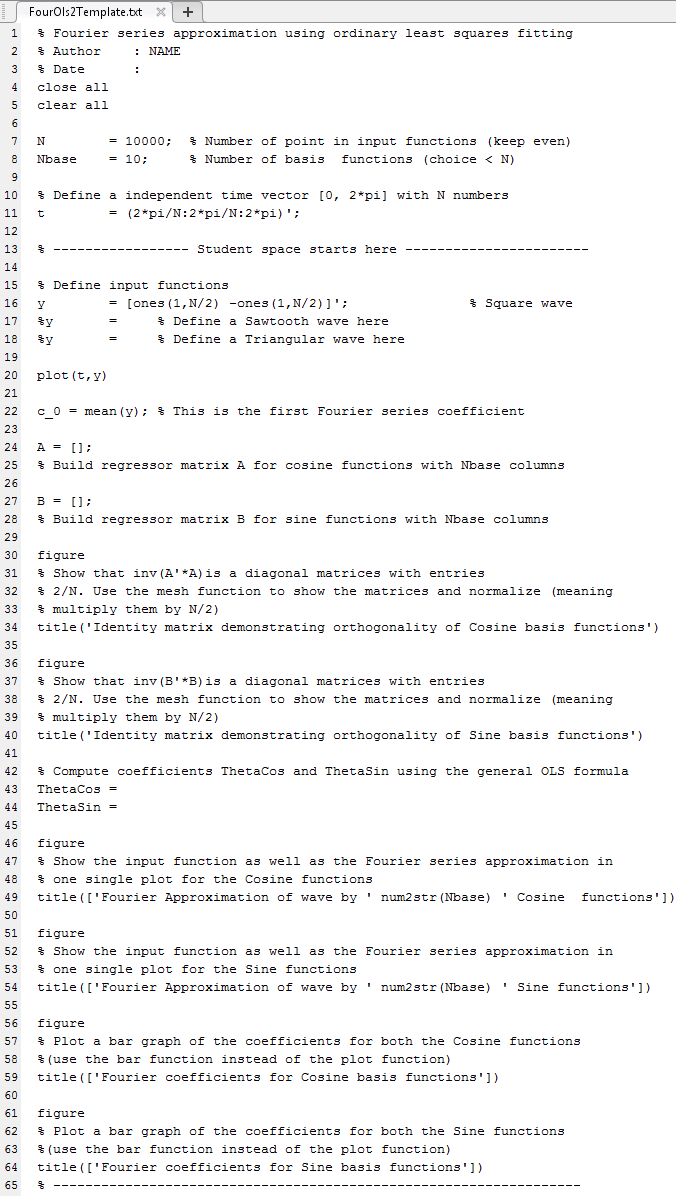
\includegraphics[width=0.7\linewidth]{Lab7_FourierSeriesTemplate}
\caption{OLS template to calculate the Fourier coefficients of various functions. You can download it \href{http://abe-research.illinois.edu/Faculty/grift/ABE425_2015/Labs/FourOls2Template.txt}{here}}.
\label{fig:Lab7_FourierSeriesTemplate}
\end{figure}

\begin{figure}
\centering
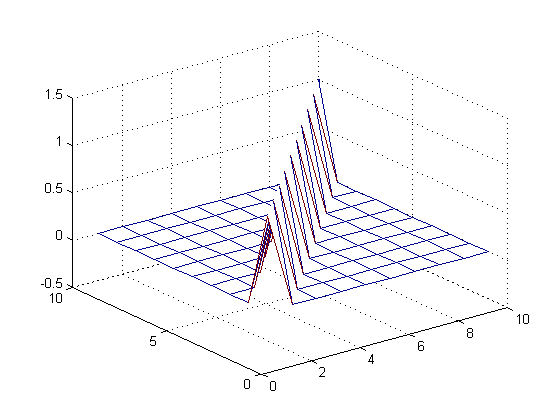
\includegraphics[width=0.8\linewidth]{Lab7_FourierSeries1}
\caption{Identity matrix showing orthogonality of sine basis functions.}
\label{fig:Lab7_FourierSeries1}
\end{figure}

\begin{figure}
\centering
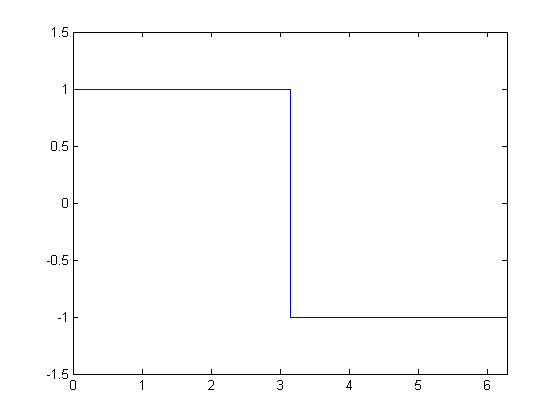
\includegraphics[width=0.8\linewidth]{Lab7_FourierSeries2}
\caption{Square wave defined on the interval $[0, 2 \pi]$.}
\label{fig:Lab7_FourierSeries2}
\end{figure}

\begin{figure}
\centering
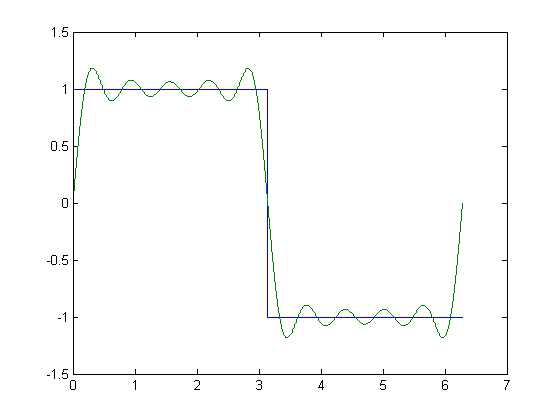
\includegraphics[width=0.8\linewidth]{Lab7_FourierSeries3}
\caption{Square wave Fourier approximation using 9 cosine basis functions.}
\label{fig:Lab7_FourierSeries3}
\end{figure}

\begin{figure}
\centering
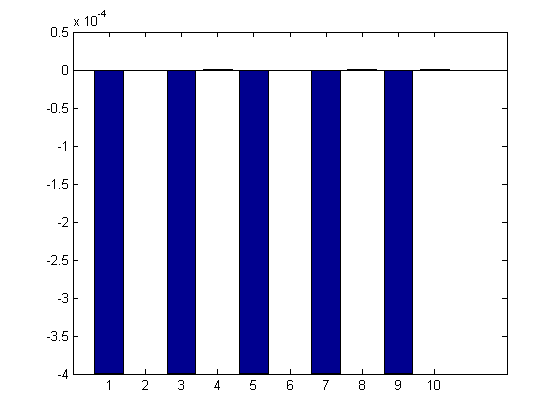
\includegraphics[width=0.8\linewidth]{Lab7_FourierSeries4}
\caption{Square wave Fourier coefficients of Cosine basis functions.}
\label{fig:Lab7_FourierSeries4}
\end{figure}

\item Define the sawtooth as shown in Figure \ref{fig:Lab7_FourierSeries6}, and run the program to find the coefficients. Paste the spectrum and approximation in your report (after Figure \ref{fig:Lab7_FourierSeries6}) move Figure \ref{fig:Lab7_FourierSeries7} to Figure 10.\\

\begin{figure}
\centering
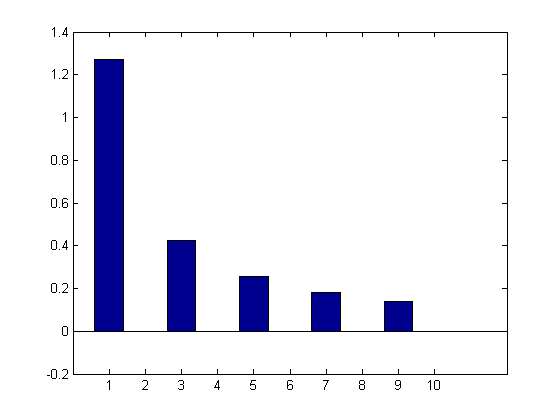
\includegraphics[width=0.8\linewidth]{Lab7_FourierSeries5}
\caption{Square wave Fourier coefficients of Sine basis functions.}
\label{fig:Lab7_FourierSeries5}
\end{figure}

\item Define the triangular signal shown in Figure \ref{fig:Lab7_FourierSeries7}, and run the program to find the coefficients. Paste the spectrum and approximation in your report.\\

\begin{figure}
\centering
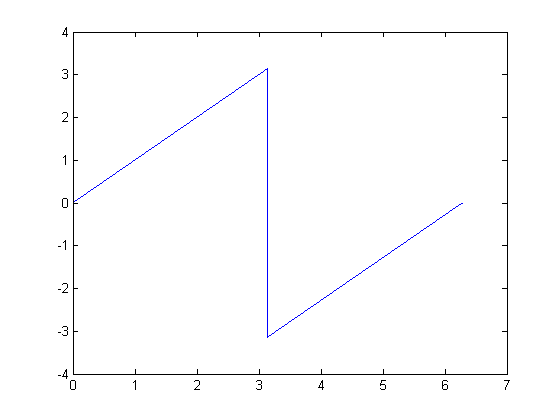
\includegraphics[width=0.8\linewidth]{Lab7_FourierSeries6}
\caption{Shown is a sawtooth function, define it and use your program to calculate the Fourier coefficients.}
\label{fig:Lab7_FourierSeries6}
\end{figure}

\begin{figure}
\centering
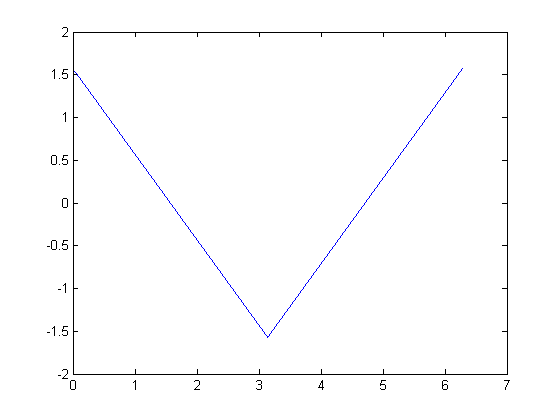
\includegraphics[width=0.8\linewidth]{Lab7_FourierSeries7}
\caption{Shown is a triangular function, define it and use your program to calculate the Fourier coefficients.}
\label{fig:Lab7_FourierSeries7}
\end{figure}

\item Change the cosine basis function to sign(cos(x)) and the sine basis function to sign(sin(x)). Run your program with 100 basis functions. From the plots, can you tell if this is also an orthogonal function set? Marvel at the beauty of the mesh plots!!

\item Compute the theoretical values of the coefficients of a square wave as shown in Figure \ref{fig:Lab7_FourierSeries2} using the following expressions for a Fourier series in continuous time.

\begin{equation}\label{Lab7_FourierSeries7}
f(t) = c_0 + \sum\limits_{n=1}^{\infty} a_n \cos nt + b_n \sin nt 
\end{equation}

with coefficients:

\begin{align}\label{Lab7_FourierSeries8}
 & c_0=\frac{1}{2\pi }\int\limits_{0}^{2\pi }{f\left( t \right)dt} \\ 
 & a_n=\frac{1}{\pi }\int\limits_{0}^{2\pi }{f\left( t \right)\cos ntdt} \\ 
 & b_n=\frac{1}{\pi }\int\limits_{0}^{2\pi }{f\left( t \right)\sin ntdt}
\end{align}

Compare the values that you obtained with the values in the coefficient plots (Figures \ref{fig:Lab7_FourierSeries4} and \ref{fig:Lab7_FourierSeries5}). The coefficient plots are essentially the frequency spectrum of the function.
\end{enumerate}

\section{Questions}

\begin{enumerate}
\item The basis functions of a Fourier series form an orthogonal set. What does this mean, and how can you tell from the lab results? 
\item Explain why in the case of the Square Wave signal, the coefficients for sine basis functions have values, whereas the coefficients for cosine basis function are essentially zero.
\item In the case of the square wave and the triangular signal, even for a large number of basis functions, it is not possible to obtain a perfect approximation at the flanks (discontinuities, see Figure\ref{fig:Lab7_FourierSeries3}). What is the name of this effect (remember this, it is typically on the exam)?
\end{enumerate}
	
\end{document}